
\section{Prototype}
\label{sec:prototype}

We chose to focus our efforts on accelerometer-based applications because there exists a wide-range of such applications available on the various mobile application markets. We considered applications that use the device's camera or microphone, as they are also fairly common. However, a scenario where multiple applications are using the camera or the microphone concurrently seemed fairly unrealistic.

\subsection{Sensor Data Filters}

We implemented three types of sensor data filters (or wakeup conditions) of varying complexity. The simplest filter is based on thresholding over raw accelerometer readings. Such a filter is satisfied if the detected acceleration exceeds the threshold. However, we noticed that accelerometer data is particularly noisy. Our expectation was that a simple thresholding filter would be satisfied more frequently than necessary because of the noise present in the sensor data, potentially causing unnecessary device wakeups. Our second and third filters are based on threshold on data that has been passed through a low-pass filter in order to remove some of the noise (TODO: I think this will be confusing. I am using the word filter multiple times with different meanings). The second filter uses a computationally cheap low-pass filter based on an exponential moving average. The third filter uses a more accurate and computationally expensive low-pass filter based on Fast Fourier Transformations.

\subsection{Software Changes}

This subsection provides an overview of the API that would be available to application developers and a description of the changes that needed to be made to the operating system.
 
\subsubsection{API}

To prevent a steep learning curve, our goal was to provide an API very similar to Android's existing sensors API. Normally, in order to receive sensor data, an application needs to register a listener (i.e. an implementation of the SensorEventListener interface) for a specific sensor with Android's SensorManager. Figure \ref{fig:androidSensorCodeNormal} shows a code example of a typical application registering a listener with the Android SensorManager for accelerometer readings.

We would modify the SensorManager to include functions that take an additional parameter that specifies which wake-up condition to be used. The available types of wakeup conditions would be predefined implementation of a WakeUpCondition interface. Figure \ref{fig:androidSensorCodeModified} shows an example of the modified code to include a wakeup condition that is satisfied when the acceleration on the x-axis exceeds $12 m/s^2$.

\begin{figure*}[t]
	\begin{verbatim}
		SensorManager mSensorManager = (SensorManager) getSystemService(Context.SENSOR_SERVICE);
		Sensor mAccelerometer = mSensorManager.getDefaultSensor(Sensor.TYPE_ACCELEROMETER);
		mSensorManager.registerListener(new MySensorEventListener(), mAccelerometer);
	\end{verbatim}
	\caption{Typical usage of Android's SensorManager}
    \label{fig:androidSensorCodeNormal}
\end{figure*}

\begin{figure*}[t]
	\begin{verbatim}
		SensorManager mSensorManager = (SensorManager) getSystemService(Context.SENSOR_SERVICE);
		Sensor mAccelerometer = mSensorManager.getDefaultSensor(Sensor.TYPE_ACCELEROMETER);
		WakeUpCondition mWakeUpCondition = new MinThresholdWakeUpCondition(Sensor.AXIS_X, 12.0);
		mSensorManager.registerListener(new MySensorEventListener(), mAccelerometer, mWakeUpCondition);
	\end{verbatim}
	\caption{Usage of the SensorManager with a wakeup condition}
    \label{fig:androidSensorCodeModified}
\end{figure*}

\subsubsection{Changes to OS}

TODO

\begin{figure}[h]
	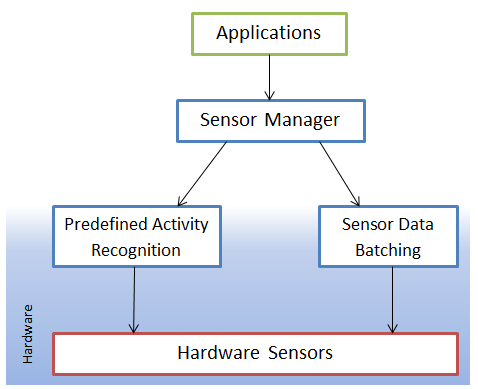
\includegraphics[width=9cm]{android_architecture_current.png}
	\caption{Simplified architecture of Android 4.4 sensor system}
    \label{fig:androidArchCurrent}
\end{figure}

\begin{figure}[h]
	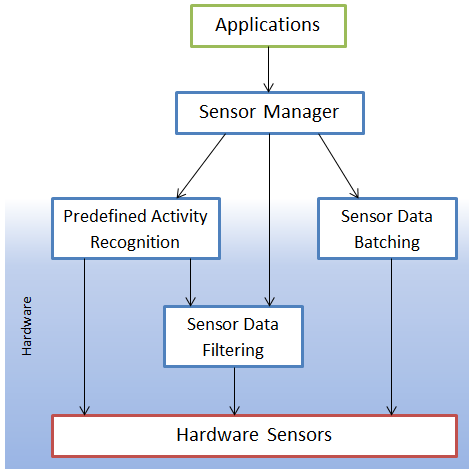
\includegraphics[width=9cm]{android_architecture_proposed.png}
	\caption{Proposed architecture based on Android 4.4 sensor system}
    \label{fig:androidArchProposed}
\end{figure}
 
\subsection{Hardware}

We evaluated two options as our low-powered sensor platform. Our first option is a Texas Instruments MSP430 micro-controller. It has the advantage of being very low-power, but it has limited memory and cannot perform complex analysis of sensor data in real-time. In our preliminary tests, the MSP430 was unable to run the Fast Fourier Transformations necessary for low-pass filtering sensor data in real-time. Our second option is a Texas Instruments Stellaris LM4F120H5QR micro-controller powered by a Cortex-M4 CPU. It can batch a higher number of accelerometer readings and perform more complex data analysis such as FFT-based low-pass filtering in real time, but it has a greater energy footprint.

TODO:Communication with Nexus 4.  Use of UART over mic port to wake up device (I'm not sure how this works)

\subsection{Power Profiles} \label{subsec:powerProfiles}

We performed power measurements on a Google Nexus 4 running Android 4.2.2. The results are summarized in Table \ref{table:powerMeasurements}. During all the measurements, the device's screen was turned off. Additionally, we noticed that changes in signal strength for GSM, WiFi and GPS resulted in fluctuations in the power consumption of the device. To prevent these factors from affecting our results, we decided to run all the power measurements with GSM, WiFi and GPS turned off.

The power measurements for both micro-controllers are also presented in Table \ref{table:powerMeasurements} on page \pageref{table:powerMeasurements}.

\begin{table*}[t]
\begin{tabular}{| l | p{7cm} | l | l |}
    \hline
    Device & State & Average Power Consumption (mW) & Average Duration \\ \hline
    TI MSP430 & Awake & 3.6 & N/A \\ \hline
    TI Stellaris & Awake & 49.4 & N/A \\ \hline
    Nexus 4 & Awake, running a pedometer application with data from the internal accelerometer & 323 & N/A \\ \hline
    Nexus 4 & Asleep & 9.7 & N/A \\ \hline
    Nexus 4 & Asleep-to-Awake Transition & 384 & 1 second \\ \hline
    Nexus 4 & Awake-to-Asleep Transition & 341 & 1 second \\ \hline
\end{tabular}
\caption{Power Measurements}
\label{table:powerMeasurements}
\end{table*}